% !TEX root = ../paper.tex

\section{Results}							% 4-5 pages

Our system captures outdoor aerial imagery, First Person View panoramas and 3D indoor point clouds.
Each intelligent quadrotor drone is under $\$500$ per unit. It has a maximum angular resolution of under $5
cm$, while the GeoEye1 satellite has an angular resolution of 41 cm; our drones are almost an order of
magnitude better. \footnote{Resolution in the context of aerial imagery is defined to be the minimum distance between two resolvable features}

\subsection{Map Stitching}

% Brief
% % Indivbidual frames from the quad are deconvoluted, removing blur
% A - process as spec'ed, slow but accurate due to SIFT
% % SIFT keypointing
% % % Corresponding keypoints
% % Overlaying maps
% Commercial Hugin processing pipeline created to use more performant stitching process where possible

Raw frames from each drone streamed from the drones for preliminary processing are overlain on Google Maps without stitching to give responders imagery as quickly as possible.

%TODO FINSIH THOUGHT!!!!
%\noindent
%For complete stitching of high resolution imagery
%\begin{enumerate}
%	\item Raw frames are sharpened to increase detail and the quality of the final stitched map
%	\item 
%\end{enumerate}
%However, this algorithm is extremely slow, a trade-off for its increased resilience.

%\noindent
%For reasonable conditions with limited motion blur, stitching work is processed with the Panotools API. \cite{Dersch:Panotools}

Photos are stitched together into full maps with the computer vision library OpenCV \cite{OpenCV:HomePage}. Features are matched with the Scale-invariant feature transform (SIFT). The process can be slow and imperfect, although optimizations are made using the drone flight plan.

Stitched maps: \autoref{fig:KennedySidewalk}, \autoref{fig:DebrisEarth}, \autoref{fig:Playground}, \autoref{fig:HouseStitch}

\subsection{Panoramic Imaging Spheres}
At clusters of image key points, a drone descends to a low altitude and spins in a complete circle while records footage with the $720$p front camera. Frames from this video are stitched together, creating a $360^{\circ}$ panoramic sphere of an area (\autoref{fig:BackyardPanoStitch}, \autoref{fig:StellingStitch} in Illustrations). \textbf{Objects as small as 5 cm are discernible in this panorama, an order of magnitude better than satellite imagery.}
\begin{figure}[H]
  \caption{Full panorama from a backyard sweep}
  \label{fig:BackyardPanoStitch}
  \centering
    \includegraphics[width=\textwidth]{illustrations/maps/backyard_pano_mag}
\end{figure}

\subsection{Face Detection}
\textbf{BRIEF:} Faces are detected within generated panoramas with a two pass algorithm we designed to manage large images. \textbf{Much of the search process in disaster recovery can be automated with our system.}

Facial features are discernible in the panoramic imaging spheres generated by low altitude drones searching for survivors. In order to eliminate the time consuming search process disaster responders must manually do even with aerial imagery, faces are detected and reported to rescuers. We evaluated three existing implementations of face detection algorithms for accuracy over a set of 39 images: the Haar feature detection in OpenCV, the FindFaces Mathematica function and Chan Vese image binarization.

\begin{figure}[h]
	\begin{minipage}{.33\textwidth}
		\caption{ChanVeseBinarize}
		\centering 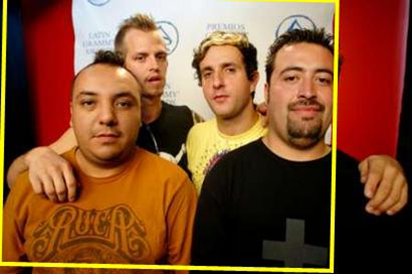
\includegraphics[width=0.95\linewidth]{illustrations/faces/1/ChanVese}
		\centering 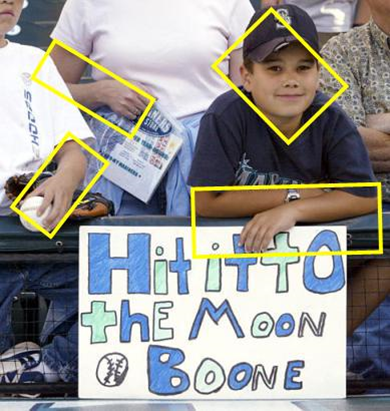
\includegraphics[width=0.95\linewidth]{illustrations/faces/2/ChanVese}
	\end{minipage}
	\begin{minipage}{.33\textwidth}
		\caption{Haar-Feature detection}
		\centering 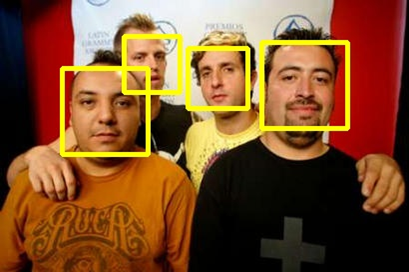
\includegraphics[width=0.95\linewidth]{illustrations/faces/1/Haar}
		\centering 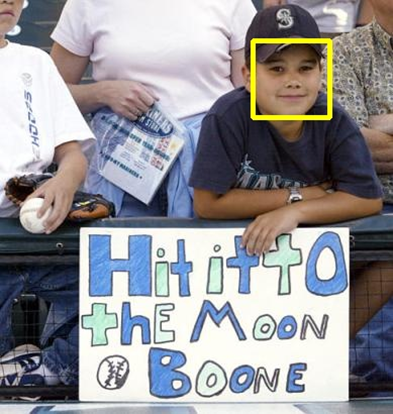
\includegraphics[width=0.95\linewidth]{illustrations/faces/2/Haar}
	\end{minipage}
	\begin{minipage}{.33\textwidth}
		\caption{FindFaces}
		\centering 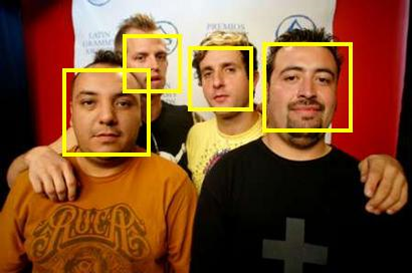
\includegraphics[width=0.95\linewidth]{illustrations/faces/1/FF}
		\centering 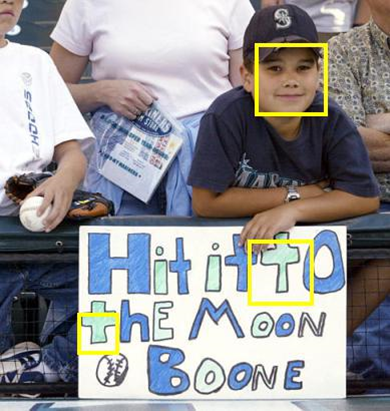
\includegraphics[width=0.95\linewidth]{illustrations/faces/2/FF}
	\end{minipage}
\end{figure}

\begin{figure}[H]
  \caption{Face detection algorithm accuracy comparison}
  \label{fig:FaceDetectionComparison}
  \centering
    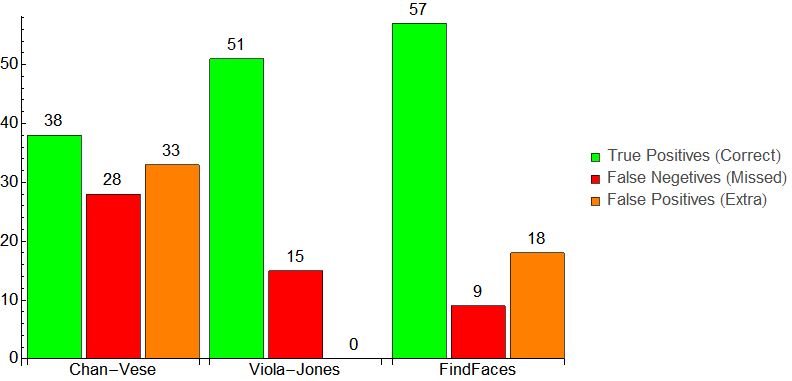
\includegraphics[width=\textwidth]{illustrations/faces/chart}
\end{figure}

\subsubsection{FindFaces and Viola-Jones}

Large XML files are distributed with OpenCV describing pre-generated Haar features. These are created ahead of time with a machine learning algorithm where faces are manually selected in a large data set. The Haar feature detection functions in OpenCV implement the Viola-Jones object detection algorithms. Other features\textemdash trees, eyes, and animals, for example\textemdash can be detected trivially by swapping out the data set.

FindFaces and the Haar feature detection method had few false positives and negatives (extra and missed faces) (\autoref{fig:FaceDetectionComparison}), but perform badly on large images. The image is usually scanned region by region, which is infeasible for our panoramas.

\subsubsection{Chan Vese Image Binarization}

The Chan Vese algorithm segments (splits) an image, locating the boundaries of an image. In the Mathematica ChanVeseBinarize implementation\cite{Wolfram:ChanVese}, objects of a target color are segmented out. By targeting skin tones, specifically orange, we were able to detect exposed skin in an image. Used exclusively for face detection, the algorithm returns many false positives since all skin and orange objects are identified. However, the algorithm can process large images far faster than Haar feature detections and FindFaces. \textbf{To detect faces in large panoramas, we first narrow the possible search space to skin colored areas with ChanVeseBinarize, then apply one of the more robust algorithms to reduce false positives.}

\subsection{3D Point Cloud Generation}

\begin{figure}[h]
	\begin{minipage}{.5\textwidth}
		\caption{Depth map created by RGBD camera.}
		\label{fig:KinectDepth}
		\centering
			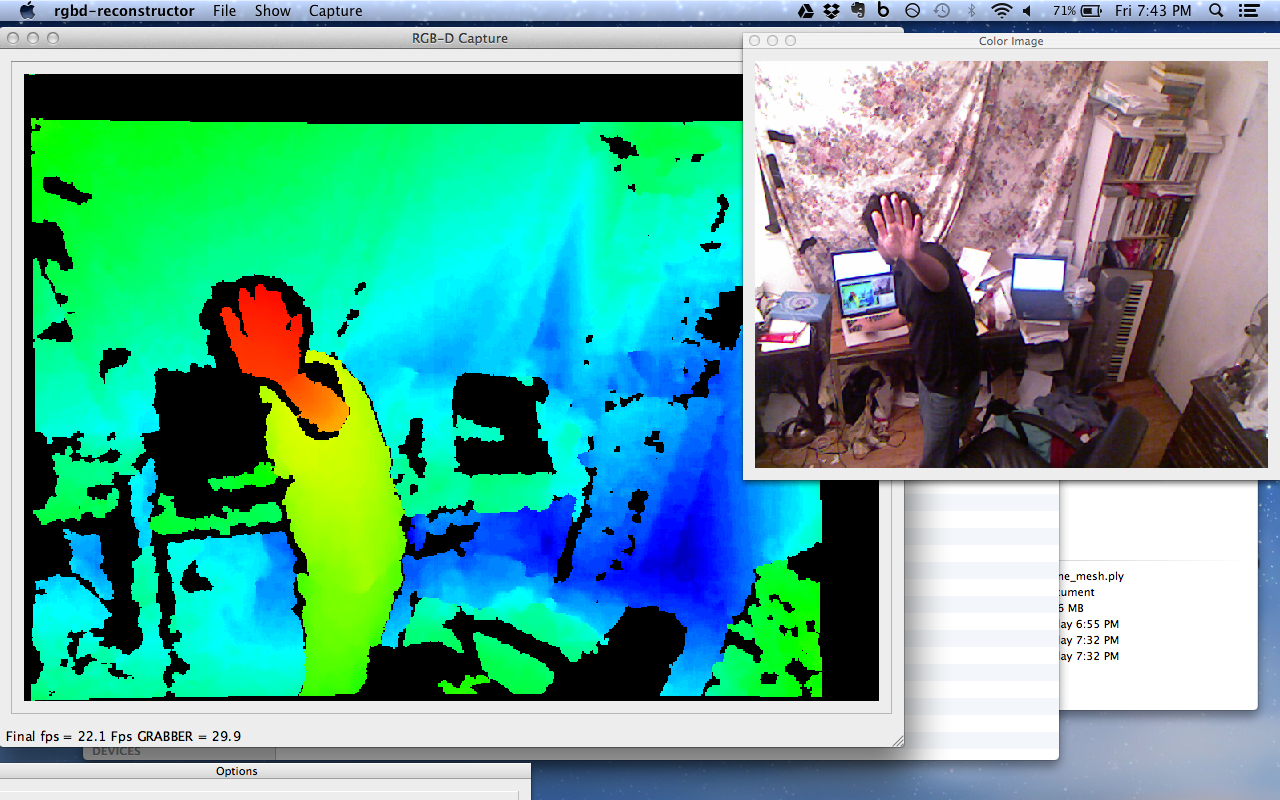
\includegraphics[width=.95\linewidth]{illustrations/clouds/depth}
	\end{minipage}
	\begin{minipage}{.5\textwidth}
		\caption{Generated point cloud. 3D map can be sent to doctors for remote diagnosis of victims.}
		\label{fig:BedPointCloud}
		\centering
			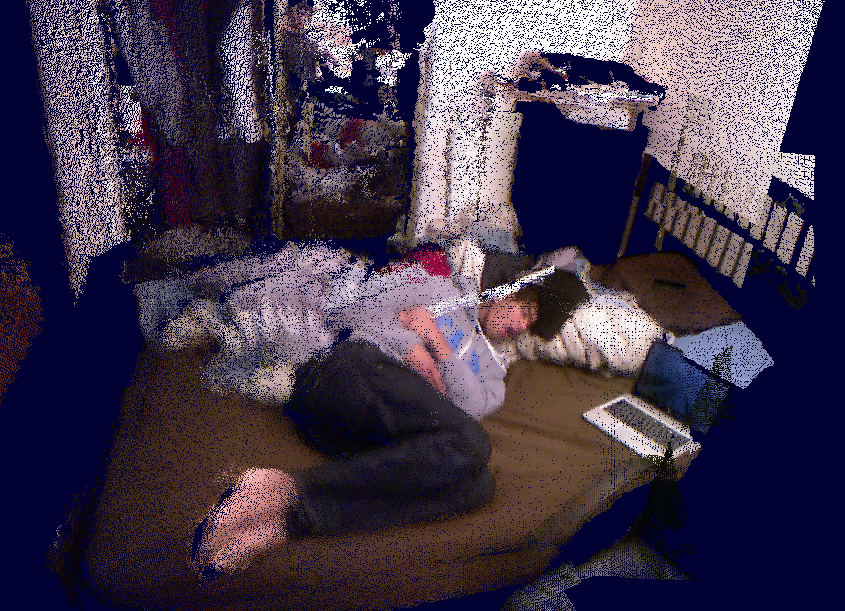
\includegraphics[width=.95\linewidth]{illustrations/clouds/bed}
	\end{minipage}
\end{figure}

Using a stripped down Asus Xtion, a consumer depth camera originally intended for gaming, RGB-D data could be obtained from an drone indoors with limited range (\autoref{fig:KinectDepth}). SLAM (Simultaneous Localization and Mapping) is used to generate 3D point clouds of the interior of a building (\autoref{fig:BedPointCloud}). \textbf{These point clouds can be sent to off-site doctors for remote diagnosis of victims. First responders do not need to enter dangerous collapsing buildings after a disaster until they are certain there is someone in need inside.}

%\begin{figure}[H]
%	\caption{Ground based tether for 3D camera due high bandwidth requirements (400mbps)}
%	\centering
%		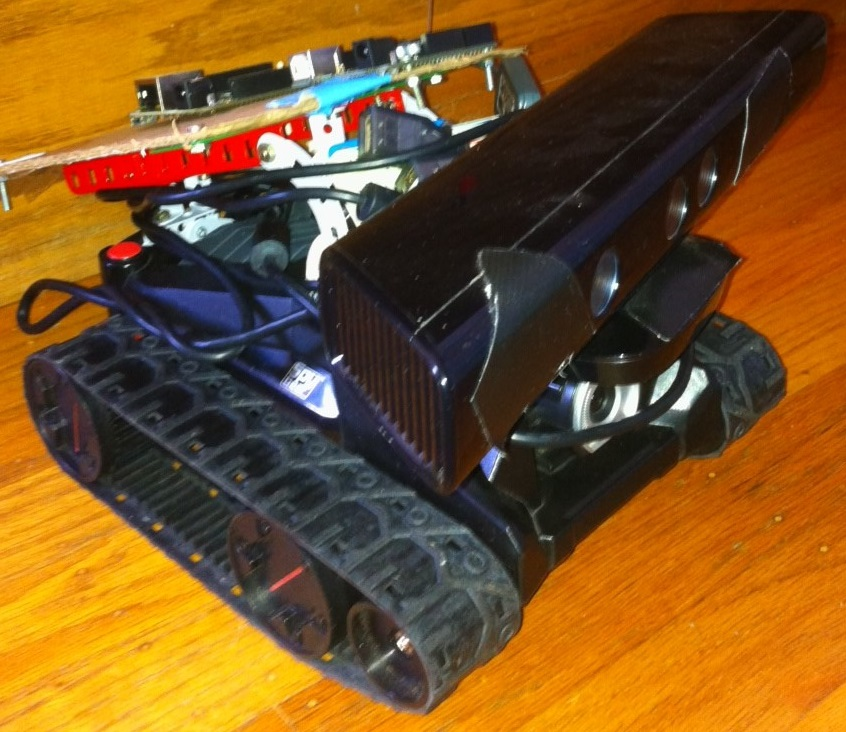
\includegraphics[width=0.5\textwidth]{illustrations/ground}
%\end{figure}

\subsection{Google Earth Map Creation}

Map data with stiches superimposed upon Google Maps is delivered to first responders through KML export for portability and ease of use by First Responders. Pictures are overlaid on a satellite map and oriented and sized from drone telemetry.\footnote{This telemetry includes latitude/longitude, heading, bearing and altitude} \textbf{Operators and first responders can assess damage in regions and determine where help is needed while locating survivors.}
